%%%%%=== work ===%%%%%
\chapter{系统硬件设计平台}
\thispagestyle{fancy}


\section{无人机平台}


由于国内的无人机制造技术已经相当成熟,而本论文关注点在于完整搜救系统的集成化,因此并没有必要从零开始自己组建无人机平台。本论文采用的无人机平台主要是大疆创新出品的DJI M100和DJI M600。

\begin{figure}[h]
    \centering
    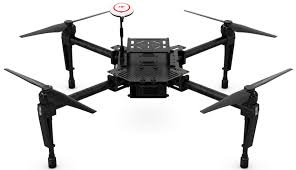
\includegraphics[height=3.43cm]{figures/3-1-M100.jpg}
    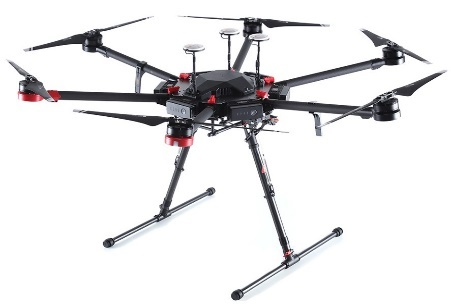
\includegraphics[height=3.43cm]{figures/3-1-M600.jpg}
    \caption{DJI M100 和 M600}\label{DJI-M100}
\end{figure}

DJI M100预留了两个UART接口,可供飞控和机载设备进行串口通信。通过UART,机载设备可以获取无人机飞行状态信息以及接收来自地面的指令。同时,为了方便开发者进行开发,DJI推出了专门的Onboard SDK开发工具包,用于提供底层的控制接口,让开发者可以专注于逻辑功能的实现。

对于本系统,机载设备完成数据处理任务,并通过UART接口将控制指令传至飞控使无人机执行相应的动作。

\section{机载计算设备}


机载计算设备采用的是Manifold。Manifold功能强大,功耗低,体积小,因此十分适合用作无人机机载计算设备。在本系统中,Manifold将运行整个无人野外搜救系统的所有逻辑功能,主要包括双目视觉点云图获取、红外图像处理、自主避障以及自主移动降落。
\begin{figure}[h]
    \centering
    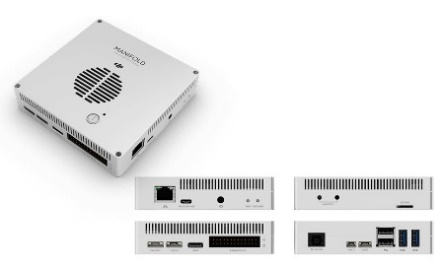
\includegraphics[height=3.43cm]{figures/3-2-Manifold.jpg}
    \caption{Manifold 妙算及其接口}\label{Manifold}
\end{figure}


\section{无人机云台相机}


无人机云台相机主要作用是获取光学航拍图像数据,用于目标搜索任务。本系统使用的是Zenmuse X3相机,X3相机可以向地面站提供1080P高清视频数据,图传距离可达$2,000m$。由于相机拍摄的图像分辨率较高,使用机载计算设备Manifold对其进行图像处理比较吃力,因此光学图像处理将在地面端进行。
\begin{figure}[h]
    \centering
    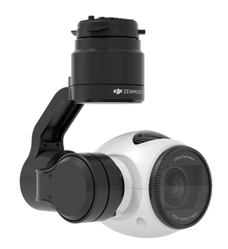
\includegraphics[height=3.43cm]{figures/3-3-X3.png}
    \caption{DJI Zenmuse X3 相机}\label{X3}
\end{figure}



\section{热成像仪}

本系统使用的是美国FLIR公司出品的FLIR VUE Pro热成像仪,其镜头大小为$19mm$,可以提供$640\times512$分辨率的红外热成像图像,其适合用于小体积、远距离和温差较小的场景,尤其是在搜索、检测等需要快速识别目标的任务中。由于此热成像仪的分辨率较小,机载计算设备Manifold可以轻易地对其进行图像处理。



\section{双目视觉模块}

系统自主避障所使用到的双目视觉模块来自于大疆公司发布的Guidance套件。 
\begin{figure}[h]
    \centering
    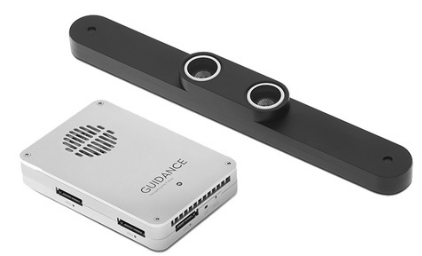
\includegraphics[height=3.43cm]{figures/3-4-Guidance.png}
    \caption{Guidance 双目视觉模块}\label{Guidance}
\end{figure}

Guidance的有效观测范围为$0.2m$到$30m$,分辨率为$640\times480$,能够满足本系统的自主避障的需求。



\section{地面站}

地面站主要包含遥控器,安卓手机和笔记本电脑。

遥控器是DJI M100配备的,其具有HDMI高清视频输出端口,可输出1080P_30FPS高清视频。笔记本电脑通过1080P高速HDMI视频采集卡读取视频流进行图像数据处理,一方面实时显示回传的无人机第一视角画面,另一方面实现地面端的目标搜索任务,与空中端的红外目标搜索组成双视频流分析,提高目标搜索的准确度和速度。

笔记本电脑性能参数如下:处理器为Intel I7-7700HQ,主频为2.8GHz,操作系统为Windows,内存为8GB ,显卡为NVIDIA Geforce GTX 1050显卡。

移动设备主要用于进行任务规划和显示无人机状态,任务规划包括设置搜索起始点,飞行速度,飞行高度等。显示无人机状况包括无人机当前飞行速度,飞行高度,GPS位置信息以及电池电量信息等。

同时,在本系统中,移动设备还充当通信中介,即手机将天空端利用红外图像处理得到的目标候选区域位置转发给笔记本电脑;以及笔记本电脑根据目标搜索的结果发送相应的指令到天空端,比如变焦相机增大减小焦距,无人机悬停拍照等。
